\subsection{Key Algorithms}
\subsubsection{DNN Selection}

The initial choice for classifying XRF spectra involved utilizing a neural network from the ResNet family, specifically ResNet50. The selection of ResNet was arbitrary but justified by its reputation as a robust CNN architecture. Notably, ResNet architecture won the ImageNet Large Scale Visual Recognition Challenge in 2015 \cite{ImageNet2015}.

ResNet architecture is characterized by its ability to support very deep networks. This is attributed to the presence of residual connections, which allow each block of network for the learning of residual mappings $g(x) = f(x) - x$ rather than the usual mapping $f(x)$ \cite{d2lResnet}. 

If the desired mapping is identity mapping $f(x) = x$, then block must only learn mapping $g(x) = 0$, which is easy to learn. 
As a result it is hard to degrade performance of this architecture with increasing depth - see \prettyref{fig:residual-block}.

\begin{figure}[h] 
  \centering     
  \includesvg[width=0.8\textwidth]{img/residual-block.svg} 
  \caption{ The residual block (right) needs to learn the residual mapping $g(x) = f(x) - x$ , wheres regular block (left) must learn direct mapping $f(x)$. Source: \cite{d2lResnet}}
  \label{fig:residual-block}
\end{figure}

However, the original architecture of ResNet incorporates a \emph{Global Average Pooling} operation just before the final fully connected layer. 
This operation calculates the average value over the spatial dimensions of a single feature map. 
In the case of adapting ResNet to work with 1D spectra, the input for global average pooling has a shape of (batch\_size, channels, features) and the output has shape (batch\_size, channels, 1). 
It means that due to averaging over features the spatial information is lost!

This resulted in the network not performing as expected, since peak positions in XRF spectra are crucial to identify elements. 
Furthermore, replacing global average pooling with a flattening operation was not feasible, as it would lead to \\ $\text{{channels}} \times \text{{features}} \times \text{{fully\_connected\_size}}$ total connections with the fully connected layer. 
For example, with an input vector of shape $(\text{{batch\_size}}, 2048, 128)$ (which was observed during development), this would result in approximately $5 \times 10^{8}$ trainable parameters, while default implementation of ResNet50 have only $\sim2.6 \times 10^7$ as a whole!

To address this problem, several possibilities were considered:
\begin{enumerate}
    \item Modifying the architecture of ResNet to further reduce dimensionality further using convolution and pooling operations.
    \item Reducing size of fully connected layer.
    \item Opting for a completely different architecture.
\end{enumerate}

While the choice of model was not crucial for this work, and size of the ResNet fully connected layer could have been easily changed, the decision was made to change used architecture completely. 
As a result, the author chose to use the ViT (Vision Transformer).

\subsubsection{Multi-Head Attention}
To understand ViT one ought to first understand how transformers work in general.
Transformer architecture was originally meant to be replacement for RNNs (Recurrent Neural Networks) \cite{Vaswani2017}.
Although transformers needs more training data (due to small inductive bias\footnote{e.g. ``In computer vision related tasks, the great success of convolutional neural networks (CNN) is often attributed to its inductive biases, such as locality and translation equivariance. \cite{Mormille2023}''. 
In contrast, transformers exhibit less inductive biases, enabling them to explore a broader hypothesis space. 
Consequently, they may converge to local optima and generalize poorly on unseen data, when trained on insufficient data.}) 
than recurrent networks to achieve similar results, they have significant advantage in terms of parallelization.

Unlike classic RNNs, which require the use of the hidden state calculated at time step $t-1$ to compute the hidden state at time step $t$, which makes them non-parallelizable, transformers are highly parallelized, thanks to \emph{Multi-Head Attention}, which makes heavy use of matrix multiplication.

Multi-Head Attention works based on \emph{attention mechanism}, which is somewhat similar to a database query \cite{d2lAttentionMechanism}.
To explain it let's define a key-value database consisting of $(\mathbf{k}, \textbf{v})$ vector pairs which can be queried using $\mathbf{q}$ vector query: \[ D\overset{\text{def}}{=}\{(\mathbf{k_i}, \mathbf{v_i}) \mid i = 1, 2, \ldots, n\}.\]
Then attention over $D$ can be denoted as:
\[ \text{Attention}(\mathbf{q}, D) = \sum_{i=1}^{n}\text{a}(\mathbf{q}, \mathbf{k_i})\mathbf{v_i},\]
where $\text{a}(\mathbf{q}, \mathbf{k_i}) \in \mathbb{R}$ are attention weights.

If exactly one of the weights $\text{a}(\mathbf{q},\mathbf{k_i}) = 1$, while all others are $0$, then attention works like normal database query and returns value of $\mathbf{v_i}$ for $\mathbf{k_i}$ that matches $\mathbf{q}$.
In case that there are multiple non-zero weights then some linear combination of vectors is retrieved. 
For deep learning applications the following properties are desirable: $\sum_i \text{a}(\mathbf{q}, \mathbf{k_i}) = 1$ and $\text{a}(\mathbf{q}, \mathbf{k_i}) \ge 0$. To guarantee this behaviour, the Softmax function can be applied:

\[ \alpha(\mathbf{q}, \mathbf{k_i}) = \text{Softmax}(\text{a}(\mathbf{q}, \mathbf{k_i})) = \frac{\text{exp}(\text{a}(\mathbf{q}, \mathbf{k_i}))}{\sum_j \text{exp}(\text{a}(\mathbf{q}, \mathbf{k_j}))}.\]

The last thing to be defined is the attention scoring function $\text{a}(\mathbf{q}, \mathbf{k_i})$.
It is highly unlikely to find any exact match between $\mathbf{q}$ and $\mathbf{k_i}$, so $\text{a}(\mathbf{q}, \mathbf{k_i})$ must be defined as some similarity function between vectors in feature space.

Let's take a look at Gaussian similarity kernel, which is non-linear function of euclidean distance:
\[\text{K}(\mathbf{x}, \mathbf{x'}) = \text{exp}(-\frac{\norm{\mathbf{x} - \mathbf{x'}}}{2\sigma}).\]
It has nice property of being bound between zero and one, unlike euclidean distance which could be anything and lead to numerical instabilities.
However, it has disadvantage of being computationally costly.

Now lets consider the kernel with substituted $\mathbf{q}$ and $\mathbf{k_i}$, exponentiation skipped, and in expanded form:

\[\text{k}(\mathbf{q}, \mathbf{k_i}) = -\frac{1}{2}\norm{\mathbf{q} - \mathbf{k_i}}^2 = \mathbf{q}^\intercal \mathbf{k_i} - \frac{1}{2}\norm{\mathbf{k_i}}^2 - \frac{1}{2}\norm{\mathbf{q}}^2.\]
The last term is constant across all values of $\mathbf{k_i}$ and due to normalization its presence don't affect the result. 
Therefore, it can be safely omitted. 
Similarly, the second term may be disregarded because batch/layer normalization effectively bounds $\norm{\mathbf{k_i}}$, ensuring a negligibly small impact on the final result \cite{d2lAttentionScoring}.

If we assume that $q \in \mathbb{R}^{d}$ and $k_i \in \mathbb{R}^d$, and that their elements are drawn from distribution $\mathcal{N}(\mu=0, \sigma^2=1)$, then their dot product will have mean zero and variance $d$.
After normalization by factor $\frac{1}{\sqrt{d}}$, the first commonly used attention function - \emph{scaled dot product attention} \cite{Vaswani2017} can be written as:

\[\text{a}(\mathbf{q}, {\mathbf{k_i}}) = \frac{\mathbf{q}^\intercal \mathbf{k_i}}{\sqrt{d}}.\]
Final attention weights can be calculated by applying Softmax: 

\[\alpha(\mathbf{q}, \mathbf{k_i}) = \text{Softmax}(\text{a}(\mathbf{q}, \mathbf{k_i})) =\frac{\text{exp}(\frac{q^\intercal k_i}{\sqrt{d}})}{\sum_j \text{exp}(\frac{q^\intercal k_j}{\sqrt{d}})}.\]

To take advantage of parallelization, vector multiplication can be replaced with matrix multiplication. When computing attention for $n$ queries and $m$ key-value pairs, where both queries and keys have a length of $d_k$ (although it must not necessarily be the case), and values have a length of $d_v$, the following matrices must be defined: $Q \in \mathbb{R}^{n \times d_k}$, $K \in \mathbb{R}^{m \times d_k}$, and $V \in \mathbb{R}^{m \times d_v}$. These matrices will form an equation analogous to that of vectors:

\[\text{Attention}(Q, K, V) = \text{Softmax}(\frac{Q K^\intercal}{\sqrt{d}})V.\]

In practice, it was found that it is advantageous to combine multiple attention pooling outputs computed in parallel. 
In theory it may lead to capturing different behaviours of attention mechanism, e.g. capturing short-range and long-range dependencies within a sequence \cite{d2lMultiHeadAttention}.


A single output of attention pooling was originally referred to by the authors as a \emph{head}. 
Multi-Head Attention can be calculated in following way: 
\[\text{MultiHeadAttention}(Q, K, V)  = \text{Concat}(head_1, head_2, \dots, head_n)W^O,\]
where $head_i = \text{Attention}(QW_i^Q, KW_i^K, VW_i^V) \in \mathbb{R}^{p_v}$, where $W_i^Q \in \mathbb{R}^{d_k \times p_k}$, $W_i^K \in \mathbb{R}^{d_k \times p_k}$, $W_i^V \in \mathbb{R}^{d_v \times p_v}$ and $W_i^O \in \mathbb{R}^{(hp_v) \times p_o}$ are learnable parameters.
To better manage computational cost, the input sizes for each head are parameterized in following manner: $p_k = p_v = p_o / h$, where $h$ is number of heads and $p_o$ is size of output of last fully connected layer. Thanks to that, computational cost don't increase with higher number of heads.

\subsubsection{ViT Architecture}
Multi-Head Attention is the most important concept used in transformer architecture, it is no different when it comes to Vision Transformer \cite{vitPaper}.
DNN architecture used to classify XRF spectra is slightly modified version of ViT, which was adapted to work with 1D input.

Most parts of the architecture remain unchanged.
Transformer encoder is implemented (\prettyref{lst:transformer_encoder}) in exactly the same way as in original paper - \prettyref{fig:transformer-encoder}.
In contrast to the original transformer encoder architecture \cite{Vaswani2017}, layer normalization in ViT is applied before all MHA and MLP (Multi Layer Perceptron) in order to enhance training effectiveness.
Moreover, the commonly used non-linear activation function ReLU (Rectified Linear Unit) is replaced with its smoother counterpart, GELU (Gaussian-Error Linear Unit).

\begin{figure}[H] 
  \centering     
  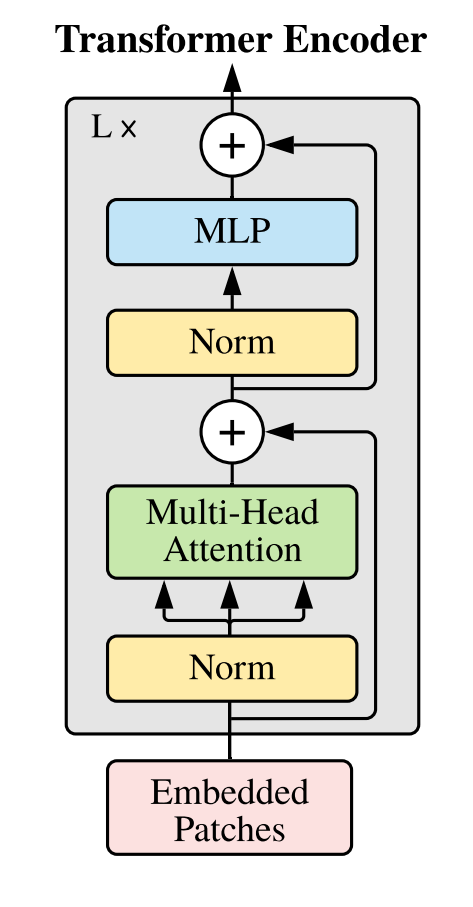
\includegraphics[width=0.3\textwidth]{img/transformer-encoder.png} 
  \caption{Transformer Encoder architecture. Source: \cite{vitPaper}}
  \label{fig:transformer-encoder}
\end{figure}

\newenvironment{longlistingA}{\captionsetup{type=listing, width=0.8\textwidth}}{}
\begin{longlistingA}
    \pythoncode{listings/transformer_encoder.py}
    \caption{Transformer Encoder block implementation. The implementation details were based on \cite{d2lViT}}
    \label{lst:transformer_encoder}
\end{longlistingA}
\vspace{12pt}

Several modifications were introduced in the remaining part of the original implementation - \prettyref{fig:original-vit-architecture}, \prettyref{fig:modified-vit-architecture}.

\begin{figure}[ht] 
  \centering     
  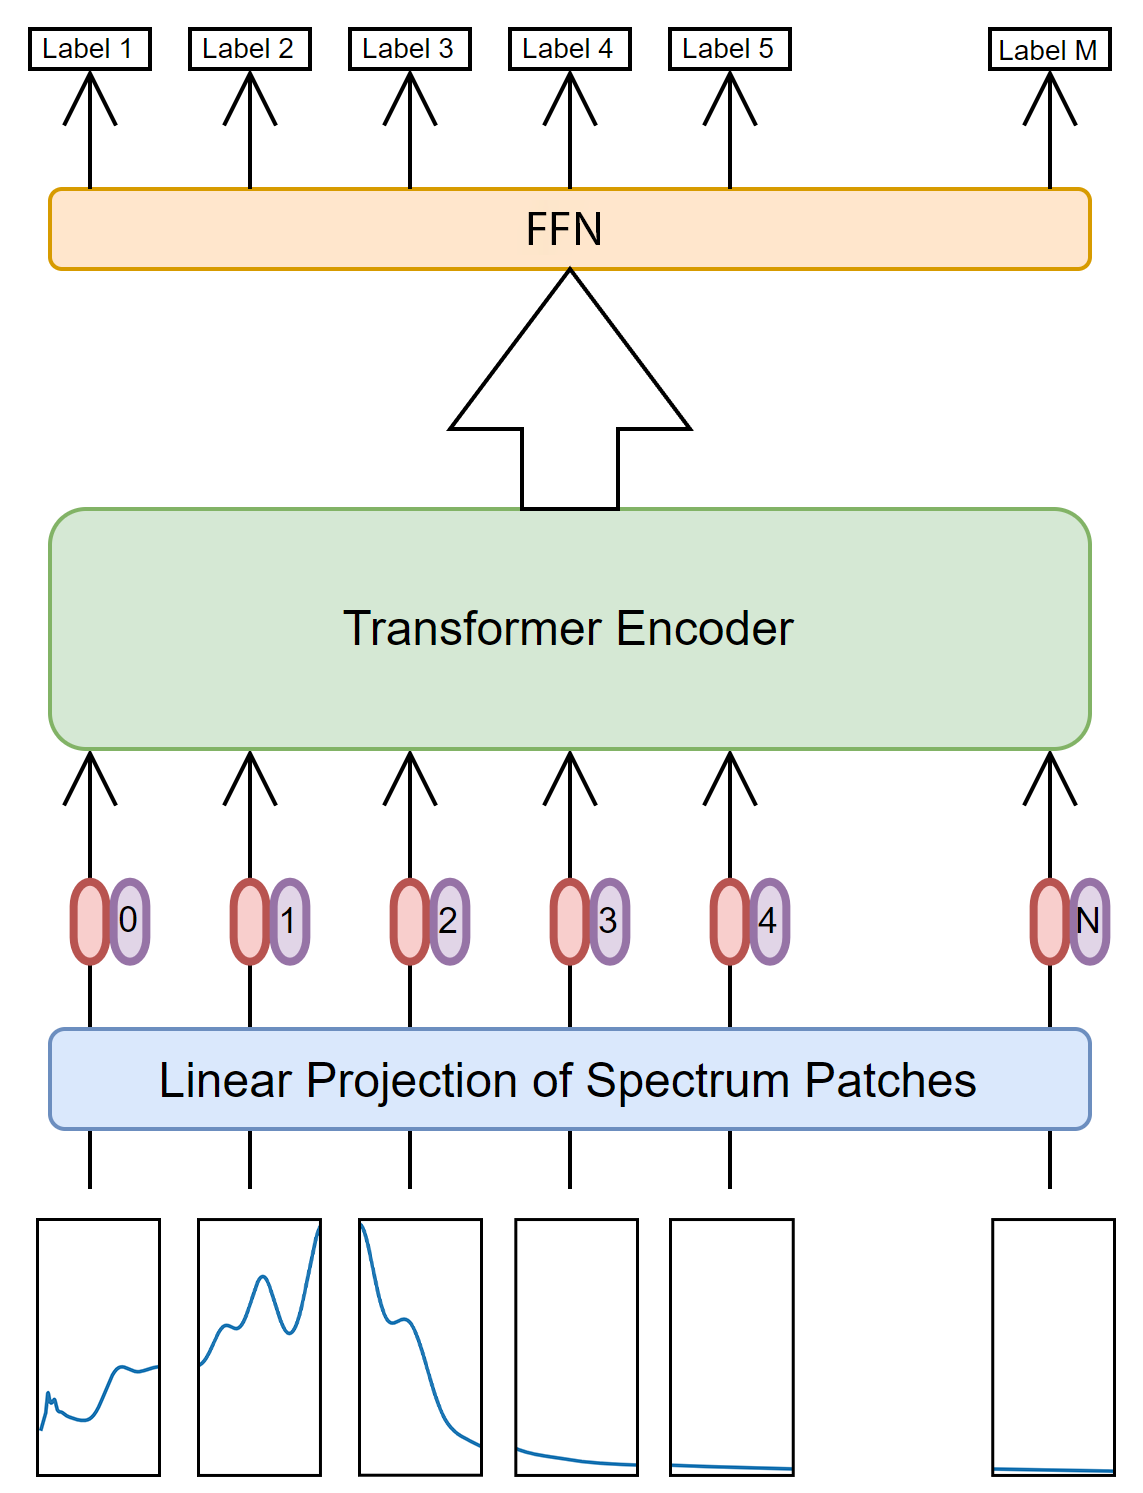
\includegraphics[width=0.6\textwidth]{img/vit_changed.png} 
  \caption{Modified ViT architecture.}
  \label{fig:modified-vit-architecture}
\end{figure}

\begin{figure}[H] 
  \centering     
  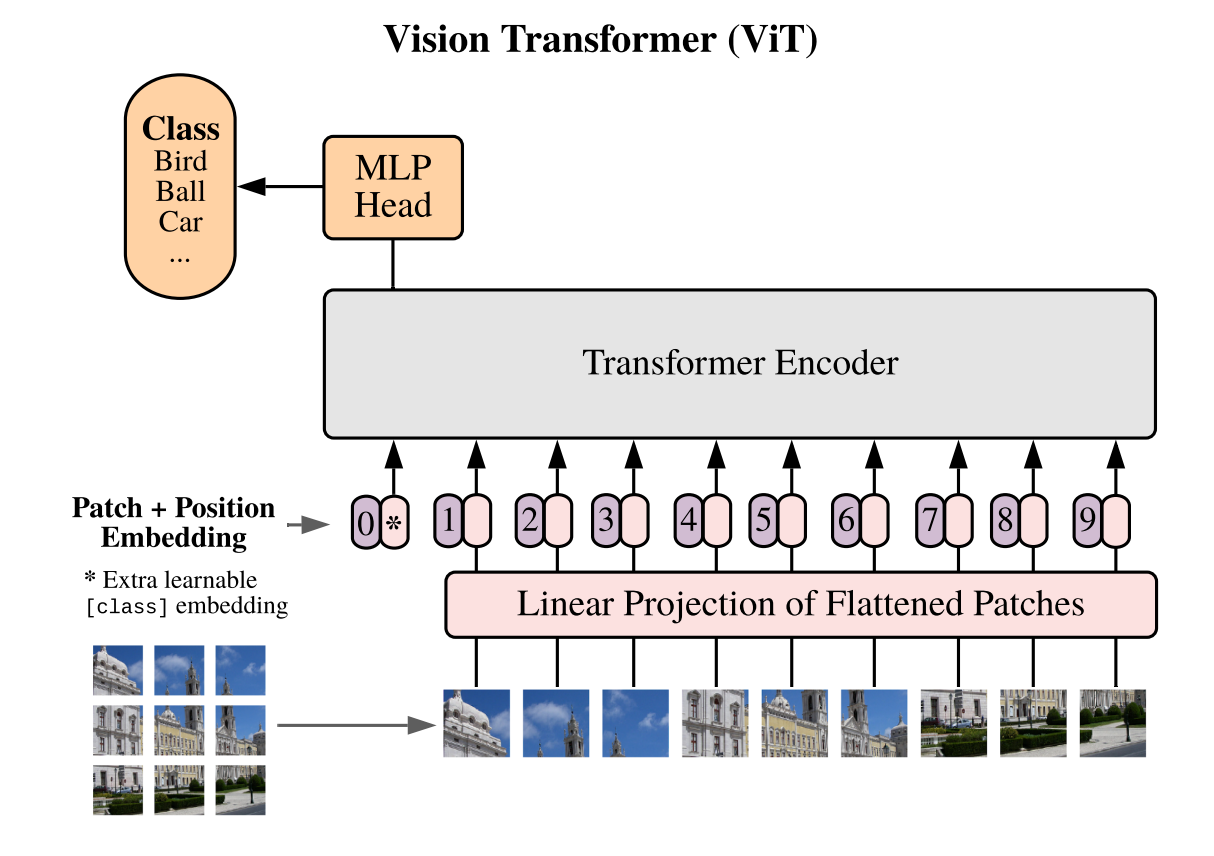
\includegraphics[width=0.7\textwidth]{img/original_vit.png} 
  \caption{Original ViT architecture. Source: \cite{vitPaper}}
  \label{fig:original-vit-architecture}
\end{figure}


The \texttt{[class]} token has been removed.
\texttt{[class]} token was an idea introduced in model BERT (Bidirectional Encoder Representations from Transformers) \cite{bertOriginal} and it was used as an input to classifying MLP.
However, due to small embedding and input size it was possible to remove it and replace with fully connected layer.
Additionally, the authors discovered that the \texttt{[class]} token was not inherently superior to other methods; other methods required just a distinct learning rate \cite{vitPaper}.

Another adjustment was to replace patch embedding using \texttt{nn.Conv2d} (2D convolution operation) with \texttt{nn.Conv1d}, because the input is not a 2D image but a 1D spectrum. 

Last but not least, the softmax function was replaced with the sigmoid function to enable the classification of multiple labels simultaneously.

\newenvironment{longlistingC}{\captionsetup{type=listing, width=0.8\textwidth}}{}
\begin{longlistingC}
    \pythoncode{listings/vit.py}
    \caption{ViT implementation. The implementation details were based on \cite{d2lViT}}
    \label{lst:vit}
\end{longlistingC}
\vspace{12pt}

\subsubsection{Self-Organizing Map}
Being able to classify elements in the spectrum is only part of the success. 
Data gathered using FF-XRF has a mean of around 20,000 photon counts per one spatial coordinate. 
When distributed over $\sim$4000 possible energy levels, it provides a rather noisy spectrum that may not yield correct classification. 
It would also come with long total inference time. 

\begin{figure}[H] 
  \centering     
  \includesvg[width=0.7\textwidth]{img/matka_boska_photon_count.svg} 
  \caption{Photon count in data gathered from the painting ``Mother of God with the Child Eating an Apple''}
  \label{fig:matka-boska-photon-count}
\end{figure}

To address this issues, one of the following strategies may be used:
\begin{enumerate}
  \item Calculating the average over small region of data.
  \item Calculating the average over clustered spectra.
\end{enumerate}

The first option is easier because clustering high-dimensional data is a daunting task due to the \emph{curse of dimensionality}.

Available options are highly limited, but they do exist. 
One algorithm that can tackle high-dimensional clustering is the SOM (Self-Organizing Map) algorithm, which is an unsupervised machine learning algorithm based on a neural network. 
It is mainly used for visualization of feature-rich data because it reduces its dimensionality to (usually) 2D map, but has been proven to work well as clustering algorithm for XRF spectra \cite{Kogou2020}.

The algorithm works in the following way \cite{somTutorial}: 
\begin{enumerate}
    \item $n$ weights $\mathbf{w_i}$ of the same length as feature vectors are initialized.
    \item Weights are distributed over a 2D map using a specified topology, such as a square, hexagonal, or random grid.
    \item A vector $\mathbf{d}$ is chosen from the training data set.
    \item $\mathbf{d}$ is compared to each node $\mathbf{w_i}$ on the map using a distance function, such as the $l_2$ norm or $l_1$ norm. The node with the closest distance is designated as the BMU (Best Matching Unit).
    \item The neighborhood of the BMU is calculated.
    \item The BMU and all nodes in the neighborhood are updated, making them more similar to $\mathbf{d}$.
    \item The algorithm is repeated from step 3 for a specified number of iterations.
\end{enumerate}

The weights are updated using following equation \cite{somWikipedia}:
\[\mathbf{w}_i^{s+1} = \mathbf{w}_i^s + \theta(u, v, s) \cdot \alpha(s) \cdot (\mathbf{d} - \mathbf{w}_i^s).\]
Here, $s$ represents the number of iterations, $u$ is the index of the BMU and $v$ is the index of the node on the map (may be the same as $u$). 
The function $\theta(u, v, s)$ represents the neighborhood function and states that the BMU is updated the most and farther neighbors are updated less. 
An example of a neighborhood function could be a Gaussian kernel. 
The function $\alpha(s)$ represents the learning rate schedule.

Although algorithm is fairly simple, the most popular python packages don't have its implementation, and the most popular implementation - package \texttt{minisom} had too large RAM memory requirements, which lead to crashing Colab environment with 50GB of memory.
Because of that its basic implementation was written using python and \texttt{numpy} package - \prettyref{lst:som}. 

\newenvironment{longlistingB}{\captionsetup{type=listing, width=0.8\textwidth}}{}

\begin{longlistingB}
    \pythoncode{listings/som.py}
    \caption{Simple Self-Organizing Map implementation. Graphical representation of weights update step can be seen in \prettyref{fig:som}}
    \label{lst:som}
\end{longlistingB}
\vspace{12pt}

\begin{figure}[H] 
    \centering     
    \begin{overpic}[width=0.6\linewidth]{img/som.png}
        \put(56,39){\textcolor{black}{\fontsize{20}{16}\selectfont $\mathbf{d}$}}
    \end{overpic}
    \caption{Updating the best matching unit (BMU) and its neighbours towards the input sample $\mathbf{d}$. Source: \cite{somGraphic}}
    \label{fig:som}
\end{figure}

\subsubsection{UMAP and HDBSCAN Clustering Pipeline}
Unfortunately, clustering the data with SOM showed some weird artifacts in all analyzed samples.
It was the reason to find alternative clusterization method to ensure that the artifacts were not caused by the algorithm.
After some research it was found that UMAP (Uniform Manifold Approximation and Projection) $\rightarrow$ HDBSCAN (Hierarchical Density-Based Spatial Clustering of Applications with Noise) clustering pipeline should also work with large datasets of high dimensional data. 

According to the UMAP documentation: ``Since UMAP does not necessarily produce clean spherical clusters something like K-Means is a poor choice. I would recommend HDBSCAN or similar. 
The catch here is that UMAP, with its uniform density assumption, does not preserve density well. 
What UMAP will do, however, is contract connected components of the manifold together. 
Providing you have enough data for UMAP to distinguish that information then you can get useful clustering results out since algorithms like HDBSCAN will easily pick out the components after applying UMAP.
UMAP does offer significant improvements over algorithms like t-SNE for clustering. 
First, by preserving more global structure and creating meaningful separation between connected components of the manifold on which the data lies, UMAP offers more meaningful clusters. \cite{umapFaq}''

Although UMAP looses in performance terms (see \prettyref{fig:umap_performance}) to PCA (Principal Component Analysis) originally used in \cite{Lach2022}, it may provide more useful dimensional embeddings because PCA is simple linear transformation, wheres UMAP is non-linear algorithm. 
\begin{figure}[htbp!] 
  \centering     
  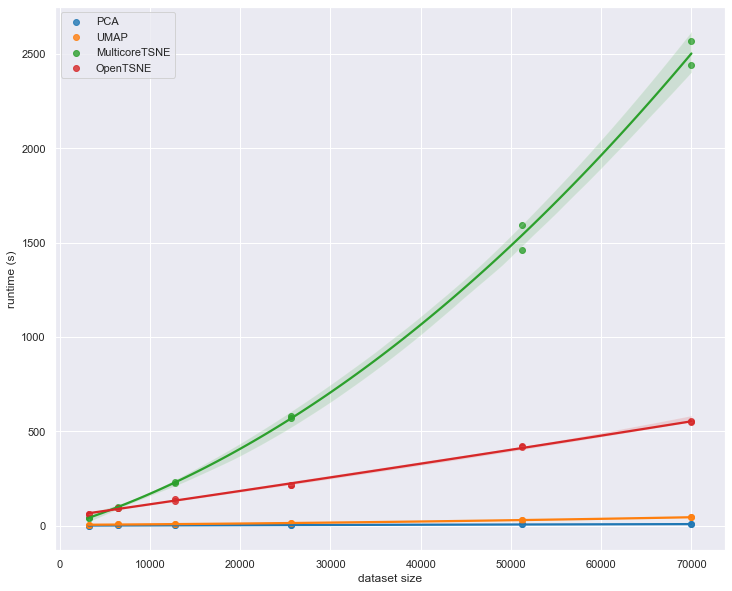
\includegraphics[width=0.8\textwidth]{img/performance_umap.png} 
  \caption{UMAP is characterized by good performance. Source: \cite{umapPerformance}}
  \label{fig:umap_performance}
\end{figure}

After dimensionality reduction using UMAP the output may be passed to HDBSCAN, which is a followup to DBSCAN algorithm.
The key difference between HDBSCAN and DBSCAN is that HDBSCAN can determine clusters with different densities.